% =========================================================================== %
% standalone document to create a scout hello world app
% =========================================================================== %
\documentclass{article}

%=============================================================================%
% Common things, settings, packages to include
%=============================================================================%

\usepackage{graphicx}
\usepackage{color}
\usepackage{makeidx}
\usepackage{ifpdf}
\usepackage{verbatim}

% --------------------------------------------------------------------------- %
% Setting up stuff depeding on output format
% --------------------------------------------------------------------------- %

\ifpdf
  % special settings for pdf mode
  \usepackage[colorlinks]{hyperref}
  \usepackage{courier}
  
  \hypersetup{
    colorlinks,
    linkcolor=darkblue,
    citecolor=darkblue,
    pdftitle={The Eclipse Scout Book},
    pdfauthor={The Scout Community},
    pdfkeywords={Enterprise Framework, Eclipse, Java, Client-Side, Rich Client, Web Client, Mobile},
    pdfsubject={Computer Science}
  }
  
  \usepackage{caption}
  \captionsetup{margin=10pt,font=small,labelfont=bf}
\else
  % special stuff for html mode
  \usepackage[tex4ht]{hyperref}
\fi

% --------------------------------------------------------------------------- %
% Setting up printing range
% --------------------------------------------------------------------------- %

\parindent 1cm
\parskip 0.2cm
\topmargin 0.2cm
\oddsidemargin 1cm
\evensidemargin 0.5cm
\textwidth 15cm
\textheight 21cm

% --------------------------------------------------------------------------- %
% Setting up listings
% --------------------------------------------------------------------------- %

\usepackage{listings}
 
\definecolor{darkviolet}{rgb}{0.5,0,0.4}
\definecolor{darkgreen}{rgb}{0,0.4,0.2} 
\definecolor{darkblue}{rgb}{0.1,0.1,0.9}
\definecolor{darkgrey}{rgb}{0.5,0.5,0.5}
\definecolor{lightblue}{rgb}{0.4,0.4,1}
\definecolor{lightgray}{rgb}{0.97,0.97,0.97}

\renewcommand{\lstlistlistingname}{List of Listings}

% general settings
\lstset{
  basicstyle=\small\ttfamily,
  columns=fullflexible,
  breaklines=true,
  breakindent=10pt,
  prebreak=\mbox{{\color{blue}\tiny$\searrow$}},
  postbreak=\mbox{{\color{blue}\tiny$\rightarrow$}},
  showstringspaces=false,
  backgroundcolor=\color{lightgray}
}

% settings for xml files
\lstdefinelanguage{xml}
{
  commentstyle=\color{darkgrey}\upshape,
  morestring=[b]",
  morestring=[s]{>}{<},
  morecomment=[s]{<?}{?>},
  stringstyle=\color{black},
  identifierstyle=\color{darkblue},
  keywordstyle=\color{cyan},
  morekeywords={xmlns,name,point,factory,class}% list your attributes here
}

% settings for ini files
\lstdefinelanguage{ini}
{
  morecomment=[f][\color{darkgrey}\upshape][0]\#, % # is comment iff it's the first char on the line
  stringstyle=\color{black}
}

% default settings (for java files)
\lstset{
  language=Java,
  emphstyle=\color{red}\bfseries,
  keywordstyle=\color{darkviolet}\bfseries,
  commentstyle=\color{darkgreen},
  morecomment=[s][\color{lightblue}]{/**}{*/},
  stringstyle=\color{darkblue},
}

% --------------------------------------------------------------------------- %
% cross reference macros
% --------------------------------------------------------------------------- %
\newcommand{\applabel}[1]{\label{apx:#1}}
\newcommand{\chalabel}[1]{\label{cha:#1}}
\newcommand{\seclabel}[1]{\label{sec:#1}}
\newcommand{\lstlabel}[1]{\label{lst:#1}}
\newcommand{\figlabel}[1]{\label{fig:#1}}
\newcommand{\tablabel}[1]{\label{tab:#1}}

\newcommand{\appref}[1]{Appendix~\ref{apx:#1}}
\newcommand{\charef}[1]{Chapter~\ref{cha:#1}\xspace}
\newcommand{\secref}[1]{Section~\ref{sec:#1}}
\newcommand{\lstref}[1]{Listing~\ref{lst:#1}\xspace}
\newcommand{\figref}[1]{Figure~\ref{fig:#1}\xspace}
\newcommand{\tabref}[1]{Table~\ref{tab:#1}\xspace}

% --------------------------------------------------------------------------- %
% graphics paths
% --------------------------------------------------------------------------- %
\graphicspath{
  {figures/}
  {Introduction/figures/}
}

%=============================================================================%

\graphicspath{{modules/figures/}}

\begin{document}

% --------------------------------------------------------------------------- %
\section*{Download and Install Eclipse Scout}

With your working Scout installation you are now ready to create your first Scout application. 
Go ahead and follow the ''Hello World!'' tutorial.

% --------------------------------------------------------------------------- %
\subsection*{Get the Package}
% =========================================================================== %
% TeX input file: "download and install scout"
%
% WARNING: this tex file does not compile standalone, it needs to be embedded
% in a master tex document (e.g. ScoutInstallation.tex)
% =========================================================================== %

Before you download Scout make sure that you have a working Java Development Kit (JDK) of version 7 or 8.
To download Eclipse Scout visit the official Eclipse download page.

\url{https://www.eclipse.org/downloads/}

The download page then looks as shown in \figref{scout_download}.
If the download page shows the wrong platform, manually select the correct platform in the dropdown list.

\begin{figure}
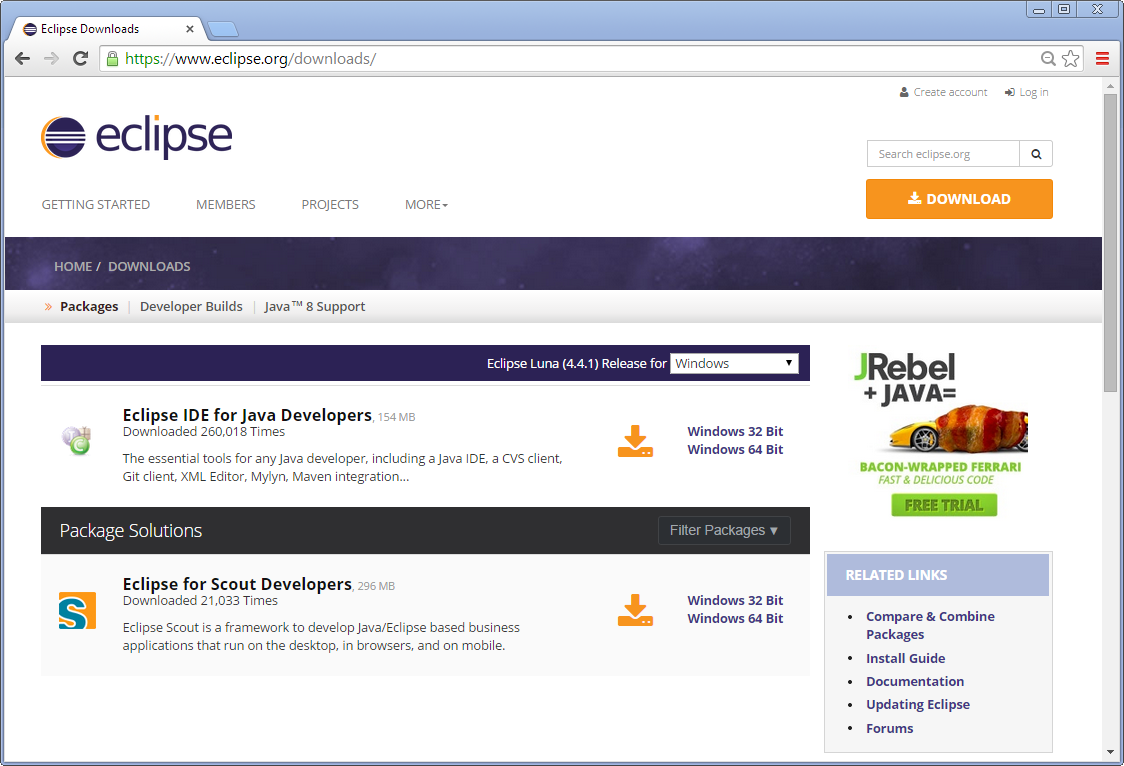
\includegraphics[width=15cm]{scout_download.png}
\caption{The Eclipse download page. The platform filter is set to Windows and the available Packages are filtered for Scout.}
\figlabel{scout_download}
\end{figure}

The Eclipse Scout package is available in the form of a 32 bit and a 64 bit package as shown in\figref{scout_download}. 
To download the correct package, make sure to matche your JDK installation. 
You can check your installation on the command line as follows.

\begin{lstlisting}[
  language=console
]
console-prompt>java -version
java version "1.7.0_55"
Java(TM) SE Runtime Environment (build 1.7.0_55-b13)
Java HotSpot(TM) 64-Bit Server VM (build 24.55-b03, mixed mode)
\end{lstlisting}

If the output explicitly mentions the 64 bit installation as shown in the example above, you have a 64 bit installation and you need to download the 64 bit Eclipse Scout package. 
Otherwise, you have a 32 bit JDK installed and you need to pick the 32 bit package of Eclipse Scout.
After the package selection, confirm the suggested download mirror as shown in \figref{scout_download_mirror}.

\begin{figure}
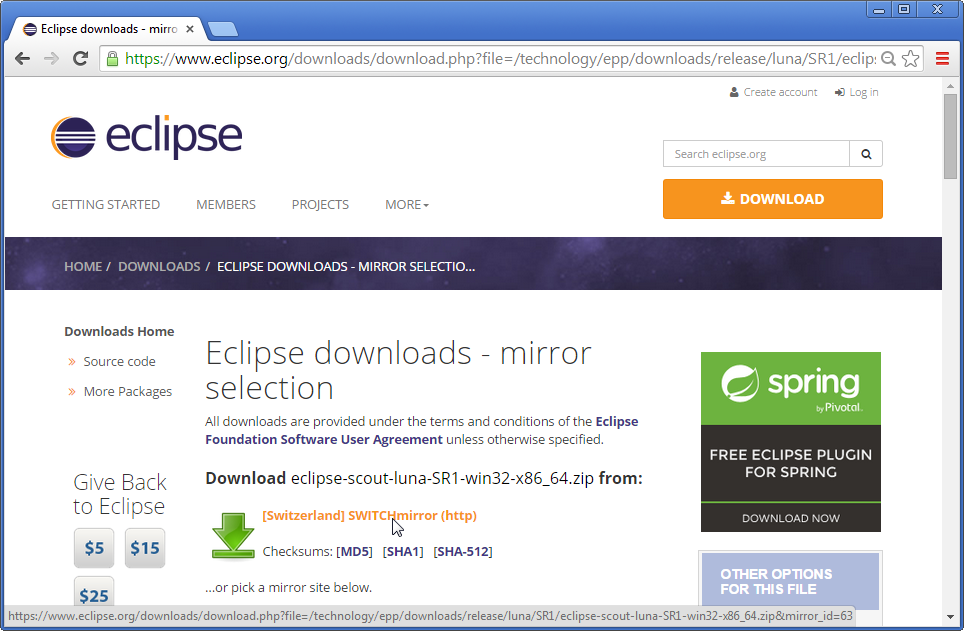
\includegraphics[width=15cm]{scout_download_mirror.png}
\caption{Downloading the Scout package from a mirror.}
\figlabel{scout_download_mirror}
\end{figure}

% =========================================================================== %
% EOF TeX input file
% =========================================================================== %

% --------------------------------------------------------------------------- %
\subsection*{Install Scout}
% =========================================================================== %
% TeX input file: "download and install scout"
%
% WARNING: this tex file does not compile standalone, it needs to be embedded
% in a master tex document (e.g. ScoutInstallation.tex)
% =========================================================================== %

As the Scout package is a simple ZIP (or tar.gz) file, you may unpack its content to a folder of your choice.
Inside the eclipse sub-folder, you will then find the Eclipse executable file, such as the \texttt{eclipse.exe} file on a Windows plattform. 
Starting the Eclipse executable brings up the workspace launcher as shown in \figref{scout_start}.

\begin{figure}
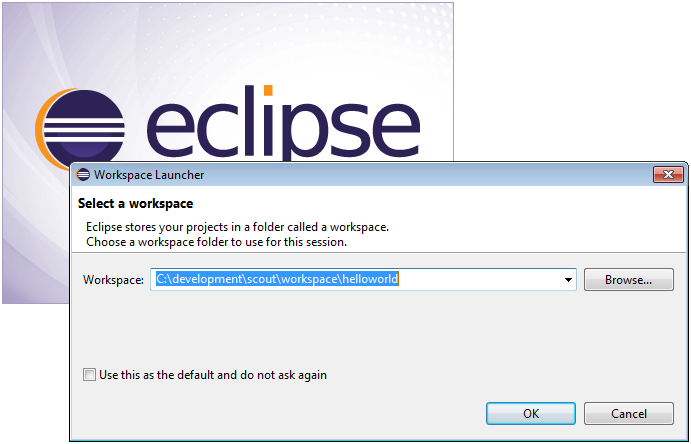
\includegraphics[width=15cm]{scout_startup_select_workspace.png}
\caption{Starting the Eclipse Scout package and selecting an empty workspace.}
\figlabel{scout_start}
\end{figure}

Into the \field{Workspace} you enter an empty target directory for your first Scout project. 
After clicking the \button{Ok}, the Eclipse IDE creates any directories that do not yet exist and opens the specified workspace. 
When opening a new workspace for the first time, Eclipse then displays the welcome screen shown in \figref{scout_welcome}. 

\begin{figure}
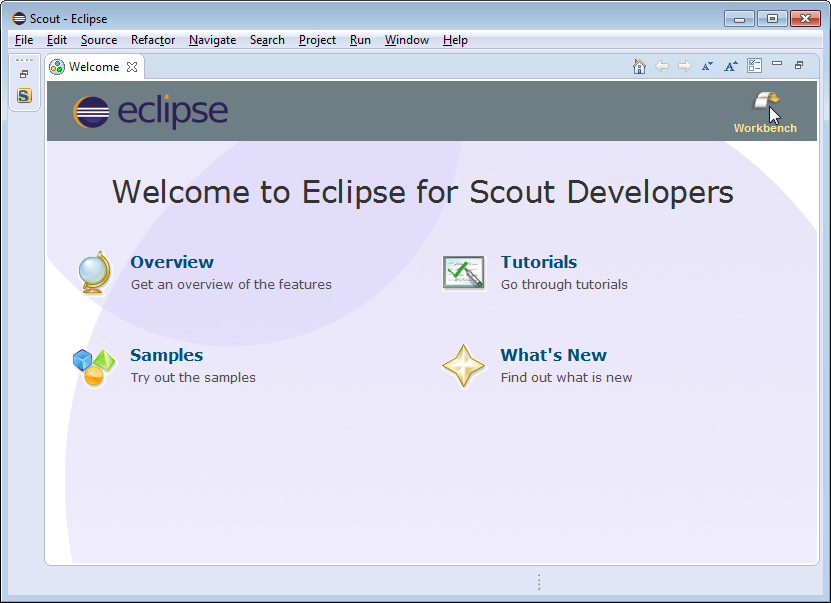
\includegraphics[width=13cm]{scout_startup_welcome.png}
\caption{Eclipse Scout welcome screen.}
\figlabel{scout_welcome}
\end{figure}

To close the welcome page and open the Scout perspective in the Eclipse IDE click on the \icon{Workbench}. 
As a result the empty Scout perspective is displayed according to \figref{scout_perspective}. 

\begin{figure}
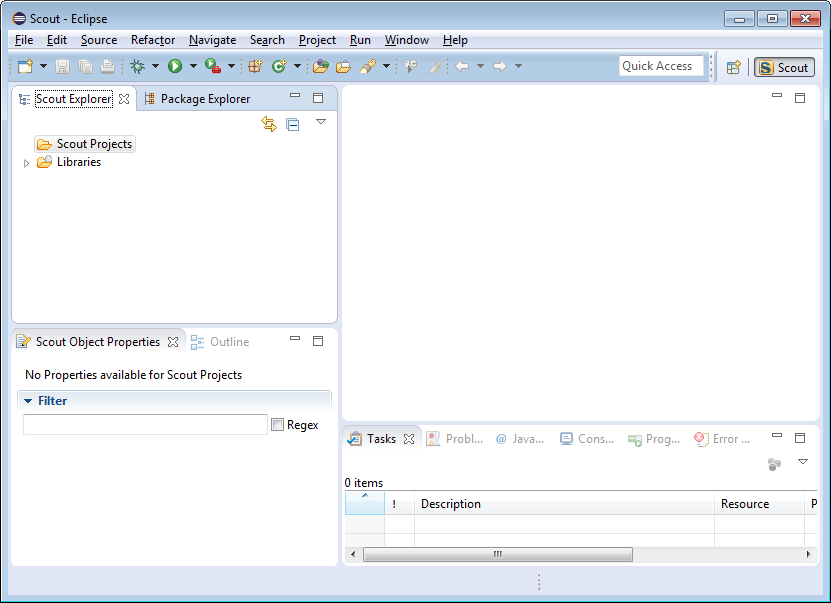
\includegraphics[width=13cm]{scout_startup_scout_explorer.png}
\caption{Eclipse Scout started in the Scout SDK perspective. }
\figlabel{scout_perspective}
\end{figure}

Congratulations, you just have successfully completed the Eclipse Scout installation!

% =========================================================================== %
% EOF TeX input file
% =========================================================================== %


% --------------------------------------------------------------------------- %
\subsection*{What's Next?}

With your working Scout installation you are now ready to create your first Scout application. 
Go ahead and follow the ''Hello World!'' tutorial.

\end{document}
% =========================================================================== %
